\chapter{Implementation and Evaluation}
\label{chap:implementation}

We implement a prototype of the recovery protocol in TypeScript on Node.js
to validate the design and serve as a reference implementation.

\section{System Architecture}
\label{sec:system-architecture}

The prototype consists of validators, clients, and a shared library.
Figure~\ref{fig:system-architecture} illustrates the architecture.

\begin{figure}[ht]
\centering
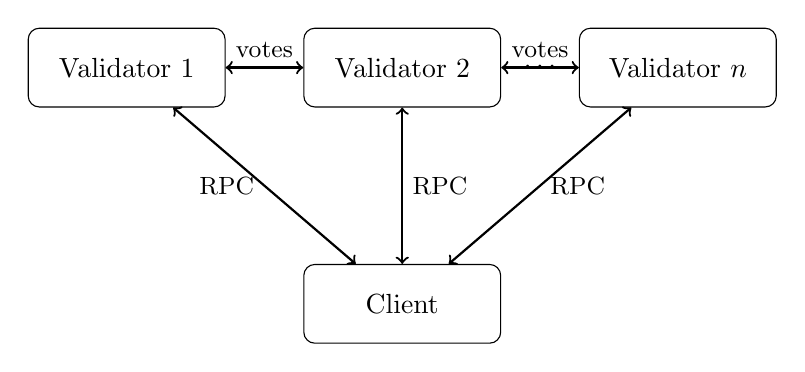
\begin{tikzpicture}[
    component/.style={draw, rounded corners, minimum width=2.5cm, minimum height=1cm, align=center},
    arrow/.style={->, thick},
    label/.style={font=\small}
]

% Validators
\node[component] (v1) at (0, 0) {Validator 1};
\node[component] (v2) at (3.5, 0) {Validator 2};
\node[component] (v3) at (7, 0) {Validator $n$};
\node at (5.25, 0) {$\cdots$};

% Client
\node[component] (client) at (3.5, -3) {Client};

% Arrows
\draw[arrow, <->] (client) -- (v1) node[midway, left, label] {RPC};
\draw[arrow, <->] (client) -- (v2) node[midway, right, label] {RPC};
\draw[arrow, <->] (client) -- (v3) node[midway, right, label] {RPC};

% Validator-to-validator
\draw[arrow, <->] (v1) -- (v2) node[midway, above, label] {votes};
\draw[arrow, <->] (v2) -- (v3) node[midway, above, label] {votes};

\end{tikzpicture}
\caption{System architecture showing validators communicating via vote propagation and clients
interacting with validators through JSON-RPC.}
\label{fig:system-architecture}
\end{figure}

\textbf{Validators.} Each validator runs as an independent HTTP server exposing
a JSON-RPC endpoint, maintaining account state (balances, nonces, pending flags)
and collected votes. On receiving a transaction, a validator checks validity,
signs a vote, and broadcasts it to all other validators.

\textbf{Clients.} Clients broadcast transactions to all validators in parallel
and collect vote responses. For recovery, clients query validators for the
current account state and construct a recovery transaction referencing the
appropriate tip.

\section{Implementation Details}
\label{sec:implementation-details}

\textbf{Transaction Format.}
The prototype uses standard Ethereum transaction format with the ethers.js
library for serialization and signing. Recovery transactions are distinguished
by their recipient: the recovery contract at \texttt{0x0...0100}, with the tip
transaction embedded in the \texttt{data} field.

\textbf{Vote Structure.}
Votes contain the validator address, account address, nonce, serialized
transaction (or null for $\bot$), and a signature over:
\[
\mathsf{message} = \mathsf{keccak256}(\mathsf{account} \| \mathsf{nonce} \| \mathsf{txHash})
\]

\textbf{State Management.}
Each validator maintains two mappings: (1) account state, mapping addresses to
$(\mathsf{balance}, \mathsf{nonce}, \mathsf{pending}, \mathsf{finalised})$
tuples; and (2) vote storage, mapping $(\mathsf{address}, \mathsf{nonce})$
pairs to collected votes. Validators check for duplicate votes to prevent
double-counting.

\textbf{Certificate Handling.}
Rather than passing explicit certificate objects between validators, the
prototype forms certificates implicitly by collecting individual votes. When a
validator accumulates $n-f$ votes for a nonce, it processes the certificate
inline, so validators only broadcast individual votes rather than assembled
certificates.

\section{Performance Evaluation}
\label{sec:performance-evaluation}

To quantify the overhead of the recovery mechanism, we compare two protocol
variants: \emph{Classic FastPay}, which implements the original protocol without
recovery, and \emph{FastPay with Recovery}, which includes the full recovery
mechanism from Chapter~\ref{chap:protocol}.

\subsection{Classic FastPay}

The classic variant omits all recovery-related code: no bot voting, no
notarisation quorum, and no recovery transactions. A validator checks only
whether $n - f$ votes have been reached for a single transaction at the current
nonce; conflicting transactions permanently lock the account.

Each protocol is configured with its maximum tolerable~$f$ for a given~$n$:
\begin{itemize}
    \item Classic FastPay: $f = \lfloor(n-1)/3\rfloor$ (the standard $3f+1$ model)
    \item FastPay with Recovery: $f = \lfloor(n-1)/5\rfloor$ (the $5f+1$ model)
\end{itemize}
Both share the same network infrastructure, cryptographic operations, and
client-side logic; the only difference is the certificate processing and the
resulting finality quorum ($n - f$).

\subsection{Benchmark Methodology}

We measure \emph{throughput} (finalised transactions per second) and
\emph{latency} (time from broadcasting a transaction to receiving $n - f$
votes). All benchmarks use $n = 12$ validators running as separate processes on
the same machine, communicating via HTTP JSON-RPC, giving $f = 3$ (quorum~9)
for Classic and $f = 2$ (quorum~10) for Recovery. Transaction signatures are
precomputed so that measurements capture only protocol execution.

\textbf{Benchmark~1: Multi-account throughput and latency.}
Each transaction uses a separate account, removing the sequential nonce
dependency. Offered load increases across phases (10, 20, 40, 80, 120,
160~tx/s), each running for 10~seconds. This measures the system's
aggregate throughput capacity. We expect both protocols to saturate at a
similar point, confirming that the recovery mechanism does not add overhead
to the happy path.

\textbf{Benchmark~2: Single-account sequential throughput.}
A single account sends transactions sequentially -- each waits for quorum and
vote submission before the next is sent. Offered load increases across the
same phases with rate limiting. This is the same setup as Benchmark~1 but
restricted to a single account, isolating the per-account throughput ceiling
imposed by nonce ordering. We again expect both protocols to saturate at a
similar point. The saturation throughput becomes the operating throughput
for Benchmark~3.

\textbf{Benchmark~3: Recovery impact on throughput.}
A single account transacts at the operating throughput identified in
Benchmark~2. After 10~seconds of steady-state operation, the client
equivocates, locking the account, then immediately recovers and resumes.
We expect throughput to dip only during the equivocation second and return
to normal immediately after.

\subsection{Results}

\textbf{Multi-account throughput and latency.}
Figure~\ref{fig:bench1-latency} shows latency as a function of achieved
throughput. At low load, both protocols achieve ${\sim}12$--$16$\,ms median
latency. Near saturation (${\sim}40$\,tx/s), latency spikes by orders
of magnitude. As expected, both protocols saturate at a similar point,
confirming that the recovery mechanism does not add measurable overhead to
the happy path.

\begin{figure}[ht]
\centering
\begin{tikzpicture}
\begin{axis}[
    xlabel={Throughput [tx/s]},
    ylabel={Latency [ms]},
    ymode=log,
    ymin=3,
    ymax=20000,
    ytick={5,10,50,100,1000,10000},
    yticklabels={5,10,50,100,1000,10000},
    width=0.85\textwidth,
    height=7cm,
    legend pos={north west},
    grid=major,
    legend cell align={left},
]
\addplot[color=TUMBlue, mark=*, thick]
    table[x=classic_tps, y=classic_median, col sep=tab] {data/bench1-latency.dat};
\addplot[color=TUMOrange, mark=square*, thick]
    table[x=recovery_tps, y=recovery_median, col sep=tab] {data/bench1-latency.dat};
\addplot[color=TUMBlue, mark=*, thick, dashed]
    table[x=classic_tps, y=classic_p95, col sep=tab] {data/bench1-latency.dat};
\addplot[color=TUMOrange, mark=square*, thick, dashed]
    table[x=recovery_tps, y=recovery_p95, col sep=tab] {data/bench1-latency.dat};
\legend{Classic (p50), Recovery (p50), Classic (p95), Recovery (p95)}
\end{axis}
\end{tikzpicture}
\caption{Latency vs.\ throughput. Solid lines show median, dashed lines show
95th percentile. Both protocols exhibit the L-curve of a saturating system.}
\label{fig:bench1-latency}
\end{figure}

\textbf{Single-account sequential throughput.}
Figure~\ref{fig:bench2-latency} shows latency for sequential single-account
transactions. As expected, latency remains flat (${\sim}9$--$13$\,ms for Classic,
${\sim}13$--$17$\,ms for Recovery) at all offered rates while actual throughput
plateaus at the per-account ceiling: ${\sim}36$\,tx/s for Recovery and
${\sim}40$\,tx/s for Classic. The
single-account ceiling is close to the multi-account saturation point from
Benchmark~1 because the Node.js event loop processes requests sequentially,
so parallel submissions offer limited additional throughput.
The saturation throughput (${\sim}36$\,tx/s) serves as the operating rate
for Benchmark~3.

\begin{figure}[ht]
\centering
\begin{tikzpicture}
\begin{axis}[
    xlabel={Throughput [tx/s]},
    ylabel={Latency [ms]},
    ymin=0,
    width=0.85\textwidth,
    height=7cm,
    legend pos={north west},
    grid=major,
    legend cell align={left},
]
\addplot[color=TUMBlue, mark=*, thick]
    table[x=classic_tps, y=classic_median, col sep=tab] {data/bench2-latency.dat};
\addplot[color=TUMOrange, mark=square*, thick]
    table[x=recovery_tps, y=recovery_median, col sep=tab] {data/bench2-latency.dat};
\addplot[color=TUMBlue, mark=*, thick, dashed]
    table[x=classic_tps, y=classic_p95, col sep=tab] {data/bench2-latency.dat};
\addplot[color=TUMOrange, mark=square*, thick, dashed]
    table[x=recovery_tps, y=recovery_p95, col sep=tab] {data/bench2-latency.dat};
\legend{Classic (p50), Recovery (p50), Classic (p95), Recovery (p95)}
\end{axis}
\end{tikzpicture}
\caption{Single-account latency vs.\ throughput. Solid lines show median,
dashed lines show 95th percentile. Latency stays flat while actual throughput
plateaus at the sequential per-account ceiling.}
\label{fig:bench2-latency}
\end{figure}

\textbf{Recovery impact.}
Figure~\ref{fig:bench3-timeseries} shows per-second throughput over time. As
expected, throughput dips only during the equivocation second and returns to
the pre-equivocation level immediately after recovery, confirming that the
recovery mechanism causes at most a one-second interruption.

\begin{figure}[ht]
\centering
\begin{tikzpicture}
\begin{axis}[
    xlabel={Time [s]},
    ylabel={Throughput [tx/s]},
    ymin=0,
    width=0.85\textwidth,
    height=6cm,
    grid=major,
    legend cell align={left},
    legend pos={south east},
]
\addplot[color=TUMBlue, thick, mark=none]
    table[x=timeSec, y=throughput, col sep=tab] {data/bench3-timeseries.dat};
\addlegendimage{dashed, TUMOrange, thick}
\addlegendentry{Equivocation}
\addlegendimage{dashed, TUMGreen, thick}
\addlegendentry{Recovery}
\draw[dashed, TUMOrange, thick] (axis cs:10.0,0) -- (axis cs:10.0,45);
\draw[dashed, TUMGreen, thick] (axis cs:10.5,0) -- (axis cs:10.5,45);
\legend{FastPay with Recovery, Equivocation, Recovery}
\end{axis}
\end{tikzpicture}
\caption{Per-second throughput during equivocation and recovery. Throughput
dips only in the equivocation second and returns immediately.}
\label{fig:bench3-timeseries}
\end{figure}

\subsection{Limitations}

These benchmarks measure a Node.js prototype, not a production system. The
original FastPay paper reports over 80,000~tx/s with 20 authorities using a
Rust implementation with native cryptographic libraries~\cite{fastpay}; our
prototype reaches roughly 40~tx/s with 12 validators -- three orders of magnitude lower. The
main bottleneck is the ethers.js signing library, which performs elliptic-curve
operations in JavaScript rather than through native bindings, adding several
milliseconds per signature. Additionally, all validators run on a single
machine communicating over localhost, so the measurements do not capture network
latency, bandwidth constraints, or geographic distribution effects that would
be present in a real deployment. A production-grade implementation and
realistic benchmarking setup are left to future work.
